%!TEX root = ../2019_7_Ozgumus_Semsi_Yigit.tex

\begingroup

This chapter presents the modifications applied to aforementioned models (see Chapter \ref{chap:sota}) to improve the
performance of the anomaly detection task. All the discussed models measures its performance metric on
well known datasets, such as CIFAR-10 \cite{cifar10} and SVHN \cite{Netzer2011ReadingDI}. The
dataset used in this thesis presents additional challenges to the anomaly detection problem we aim to 
solve. Section \ref{sec:sem} will introduce this dataset to the reader and give examples. Section \ref{sec:analysis_before} will
discuss the shortcomings of the previous models in terms of the interpretation of the dataset and
detection of the existent anomalies. Sections \ref{sec:encebgan} and \ref{sec:sencebgan} will
explain the modified architecture and the significance of the applied changes.


\section{SEM Image Dataset}
\label{sec:sem}

Nanofibrous materials acquired increasingly significant demand from variety of fields in the
Industry. It constitutes a foundation material for a lot of products including areas in medicine,
filtration, sensors and manufacturing applications \cite{carrera2016defect}. Despite the demand and
continuous research development towards its production, manufacturing nanofibrous materials is still
challenge for scaled of mass production. Several techniques for producing nanofibers have been
presented in the literature \cite{carrera2016defect}. Electro spinning method is the focus of this
anomaly detection task. It produces a structure which consists of filaments woven in with randomized
geometric pattern. You can see one of the images of the material produced without any anomalies in
Figure \ref{fig:data_norm}.

\begin{figure}[h!]
	\centering
	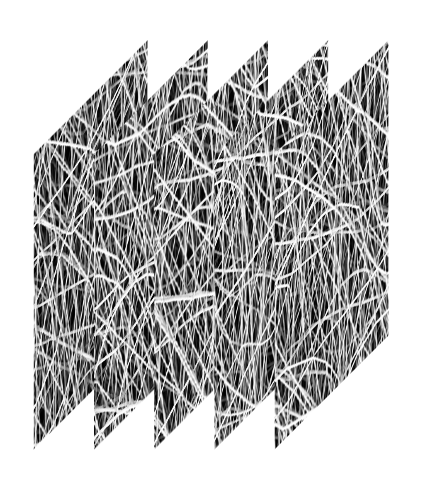
\includegraphics[width=0.75\textwidth]{dataset}
	\caption{Part of Training Dataset from the SEM Image Dataset \cite{sem}}
	\label{fig:data_norm}
\end{figure}

Scanning Electron Microscopes (SEM) Image Dataset consists of 5 images with no anomalies and 40 sample images that have various types of
anomalous regions. To preserve computational efficiency without sacrificing from performance,
training dataset and testing dataset is sampled from SEM image dataset.
\begin{figure}[h!] \subfloat[Normal regions]{
		\begin{minipage}[c][0.8\width]{0.5\textwidth}
			\centering
			\fbox{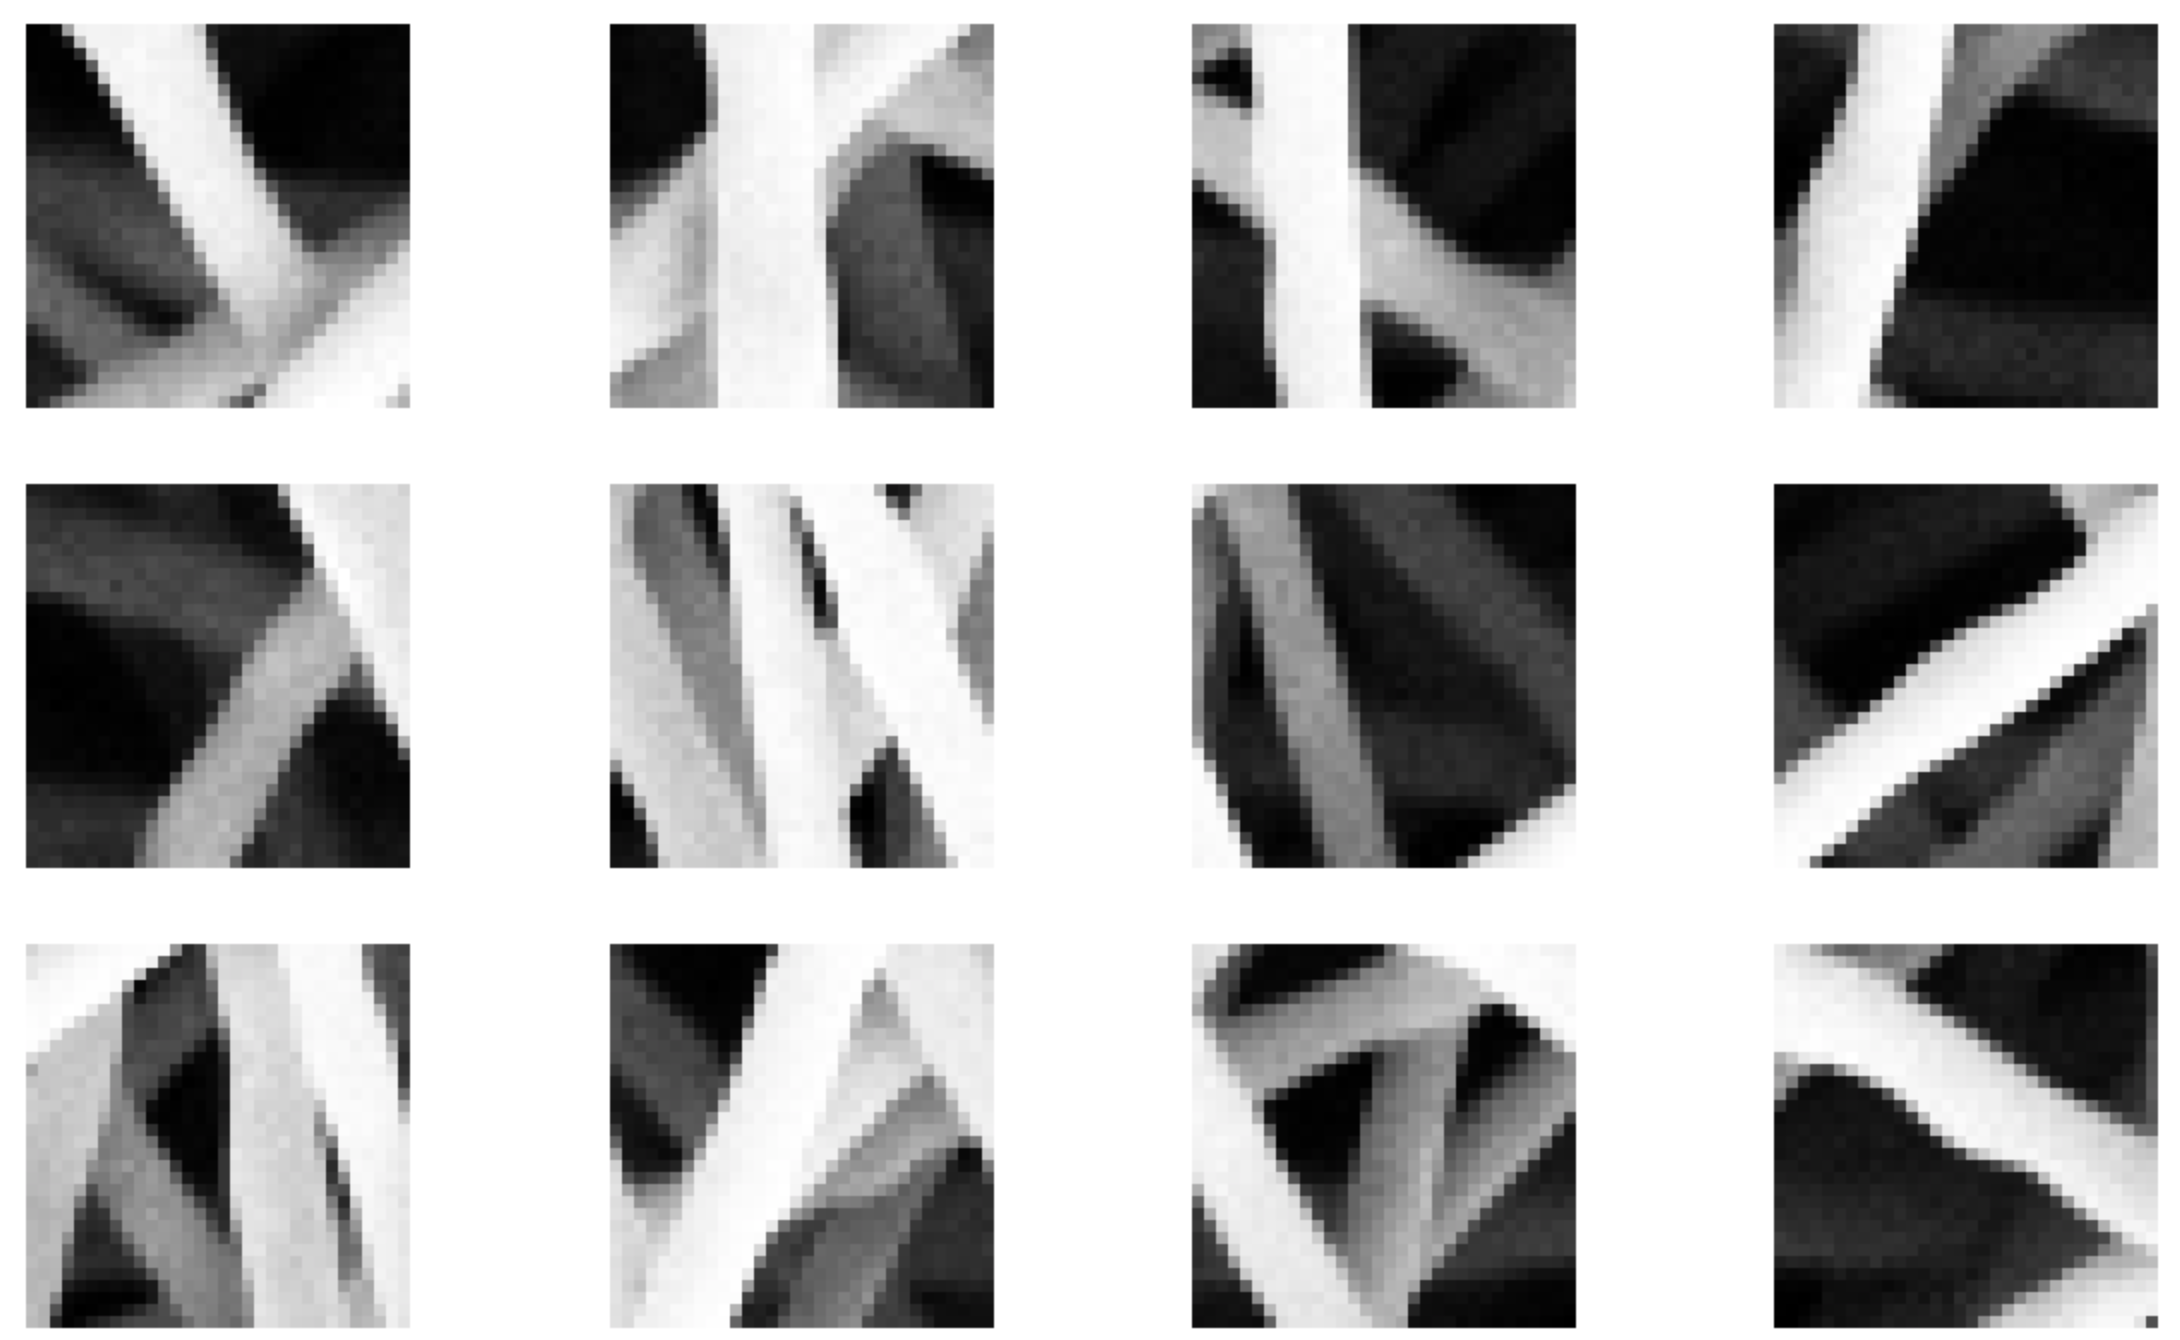
\includegraphics[width=1\textwidth]{sample_normal}}
			\label{fig:data_sample_normal}
	\end{minipage}}
	\hspace*{\fill} \subfloat[Anomalous regions]{
		\begin{minipage}[c][0.8\width]{0.5\textwidth}
			\centering
			\fbox{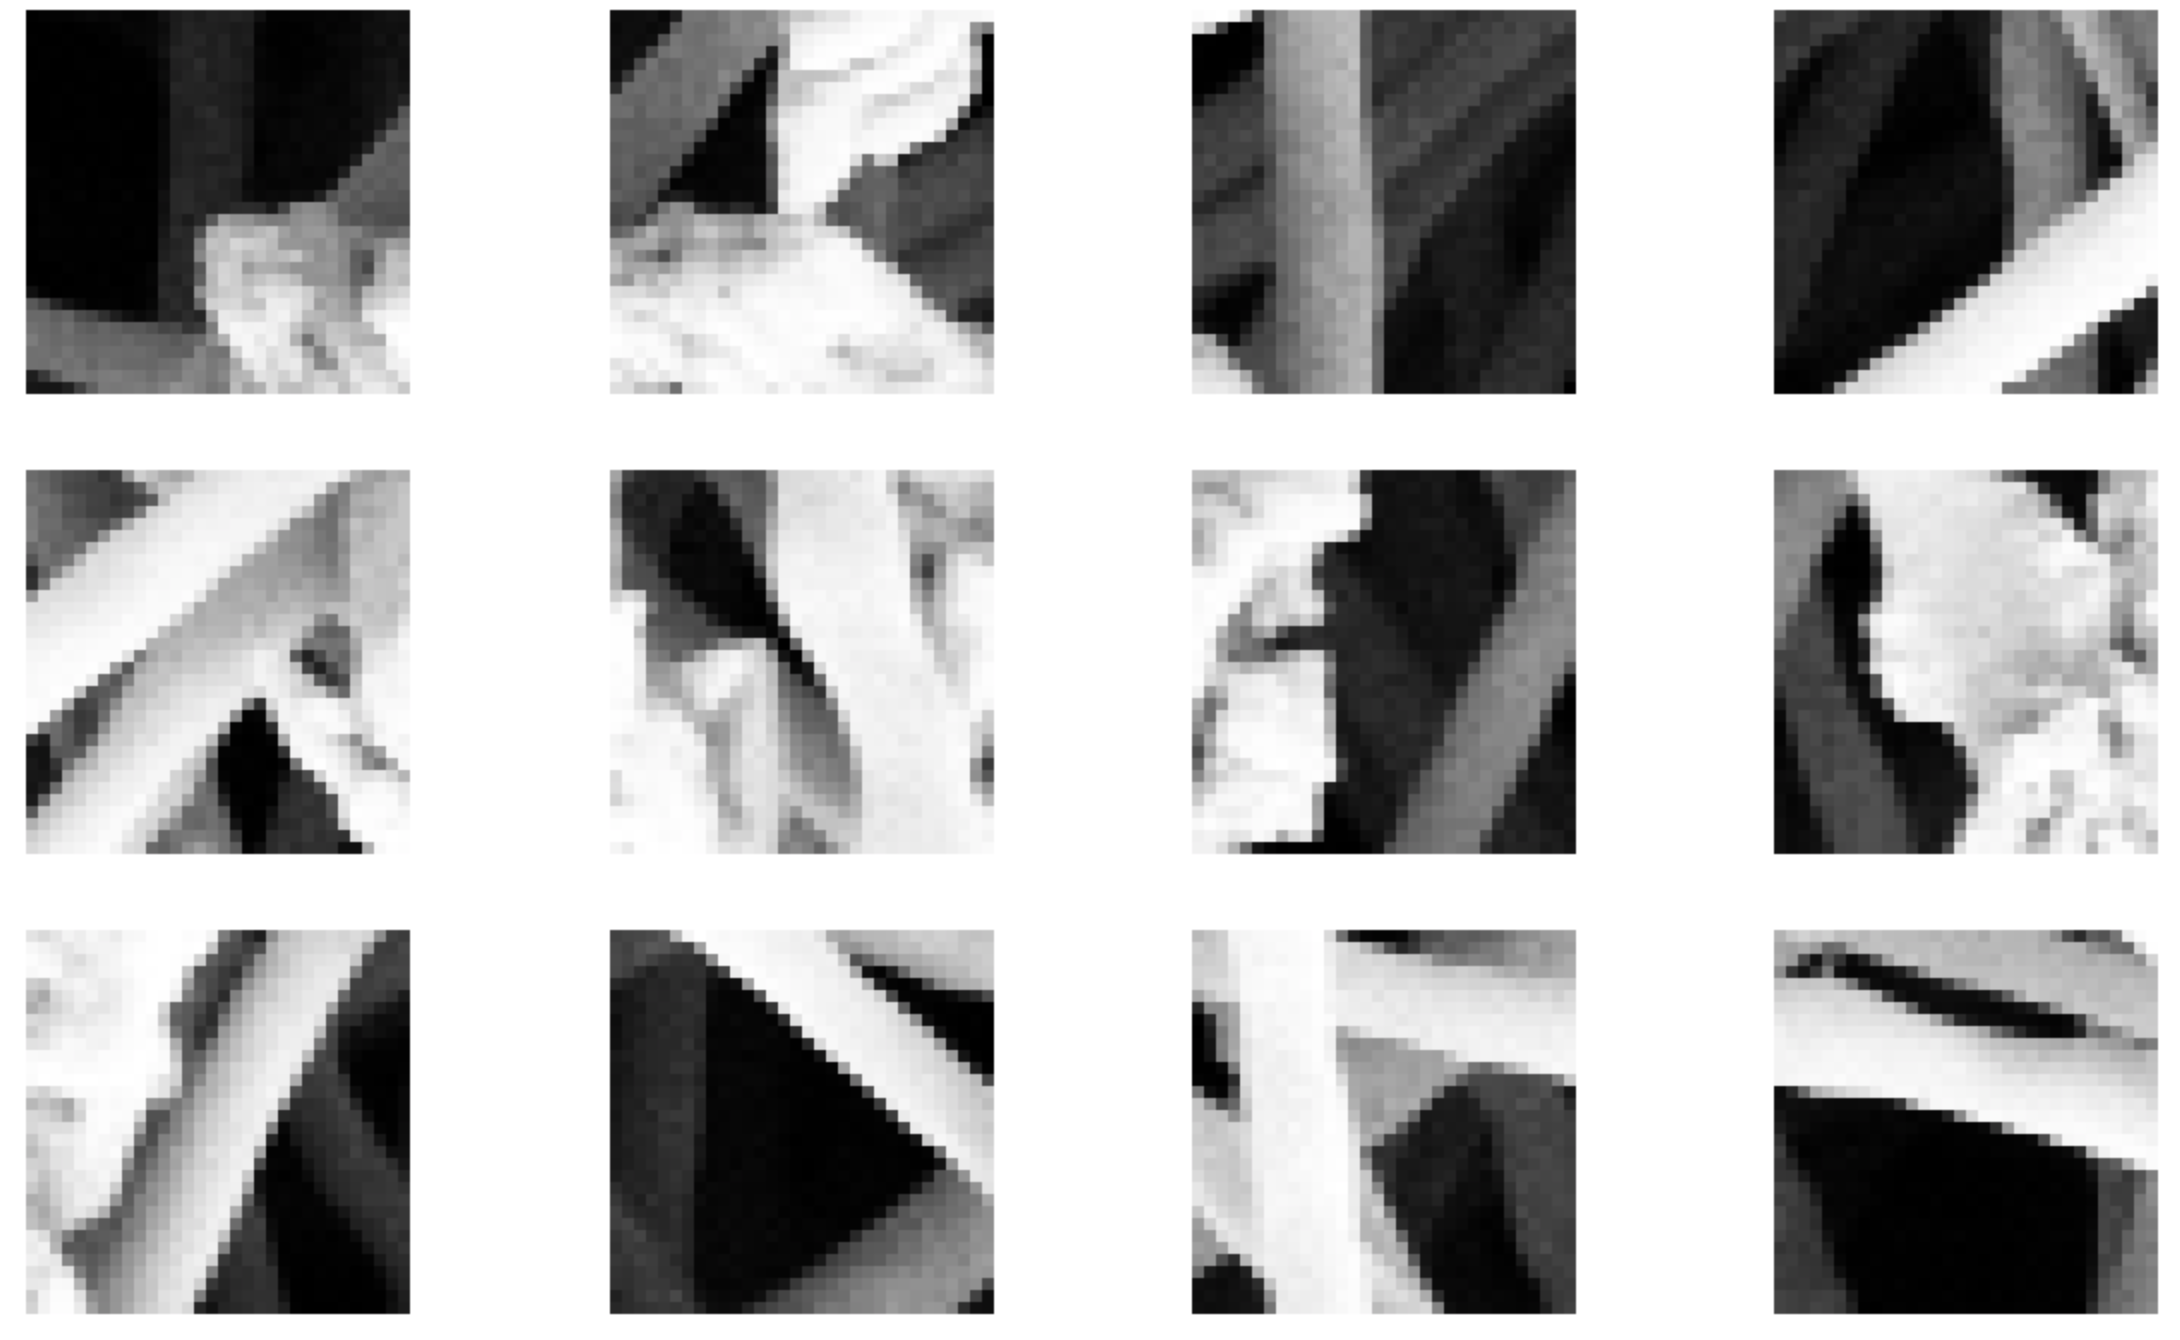
\includegraphics[width=1\textwidth]{sample_anomaly}}
			\label{fig:data_sample_anomaly}
	\end{minipage}}
	\caption{Normal and Anomalous region patches for the training and testing}
	\label{fig:data_samples}
\end{figure}

$32 \times 32$ patches are selected as the image size as if proposed framework prove useful for the
anomaly detection, testing the model with other known datasets such as CIFAR10 \cite{cifar10} and
SVHN \cite{Netzer2011ReadingDI} would be more convenient. $28 \times 28$ patch size is also
considered but choosing $28 \times 28$ image size forced model to have less transposed convolution
layers (see Chapter \ref{chap:imp_details} for model details) and GAN models designed with that
architecture experienced model collapse frequently in the preliminary experiments. Figure
\ref{fig:data_sample_normal} shows the example patches used for the training phase. Training dataset
consists of patches which contains no anomalies. Figure \ref{fig:data_sample_anomaly} shows the
anomalous samples which are used in the inference stage. Anomalous regions can reside in both
the topmost layer or can be hidden in deep in the woven structure.


\section{Analysis of Aforementioned Approaches}
\label{sec:analysis_before}

This section presents an analysis on the performance of GAN based state of the art anomaly detection
methods presented in Chapter \ref{sec:gan_based_sota} and a discussion to identify the shortcomings
of these methods. Stabilization issues in the adversarial training stage, reconstruction problems
related to the encoding of latent representation and the method of computing the anomaly score will
be discussed. While discussing these issues, our proposed model will be introduced incrementally by
addressing the modifications and measures to mitigate the affect of these shortcomings to the
performance.

Proposed models in Chapter \ref{chap:sota} can be further divided into 2 separate categories with
respect to their generator network structure. 
\begin{itemize}
	\item Pure GAN ( AnoGAN (Section \ref{sec:anogan}), BiGAN ( Section \ref{sec:bigan}) and ALAD (Section \ref{sec:alad}))
	\item Autoencoder Variants (GANomaly and Skip-GANomaly (Section \ref{sec:ganomaly}))
\end{itemize}

First group has a generator that accepts the latent noise as an input and uses adversarial training to
match the generated sample distribution to the input data distribution. The latter uses an
decoder network which used in autoencoder network in favor of the generator but still employs 
adversarial training to learn the latent representation. During the analysis of the first two problems mentioned 
which is stabilization of the generator network and convergence of the encoder network, autoencoder 
variants will not be considered for discussion since their generator network does not suffer from the
stabilization issues of GANs.


\subsection{Stabilization of Adversarial Training}

Generator and discriminator networks' objective function stabilization is still an important issue in GAN
training. Various approaches and modifications are experimented to further improve the training of
the GANs and prevent non convergent scenarios. Alternative stabilization "tricks" are proposed in 
\cite{methods} and \cite{fm} to improve the convergence properties of the objective function and prevent
mode collapse. These include adding noise with a decay over time to both input image and generated
sample before putting through discriminator to add a factor of robustness to the discriminator network,
using soft labels to define the true and fake member class instead of the binary truth values and
flipping labels of the true and generated images to fool the discriminator even more and provide
higher gradient flow to generator network early on in the training to help it learn to generate images
better \cite{fm}. 

In the training phase of a generative adversarial network, loss values of generator does not
portray a traditional convergence line in plots. Adversarial mini max game prevents the losses of the
player networks to converge to a certain limit. If the loss is reaching zero in any case, it
indicates a problem in the learning capacity of one of the networks. If discriminator network loss converges
to zero too quickly, it means that it learned to discriminate between the real images and the ones
generated by the generator network. On the other hand if the generator loss converges to zero early
in the training or experiences a sudden drops during the training it indicates a mode collapse. 
The problem is that at some point in the training generator generates an image that
perfectly fools the discriminator. If gradients obtained from this loss computation is high enough,
generator might stop learning from the gradient flow of discriminator and start to generate the same
sample in each iteration. This sample also may not be visually similar to the target distribution. Generator network 
sacrifices its diversity to increase its quality in terms of the adversarial loss.  
This essentially eliminates the purpose of having a generator network. This issue is 
tracked by observing the reconstructions from a batch of latent noise samples after each epoch of the 
training. 

To mitigate stabilization problems of generator and discriminator networks, ablation study is 
performed on all Pure GAN models which consists of previously mentioned training improvements with 
same model capacity and training hyper parameters to create an equal environment for the models. 
Despite models proving a certain performance standard on the benchmark datasets \cite{cifar10,Netzer2011ReadingDI}, 
they performed poorly on the SEM image dataset \cite{sem}. More importantly, the training of 
the networks were too unstable to obtain a consistent performance benchmark. Obtaining a stable 
GAN for generating reconstructions is fairly important because it is the first step of our anomaly 
detection framework. Figure \ref{fig:arim_training} presents the generator/discriminator learning 
graphs and their generation samples from the final training epoch.

% Figure with bigan alad anogan graphs and reconstructions
\begin{figure}[h!]
\def\tabularxcolumn#1{m{#1}}
\begin{tabularx}{\linewidth}{@{}XXX@{}}
	\begin{tabular}{ccc}
		\subfloat[AnoGAN generator training]{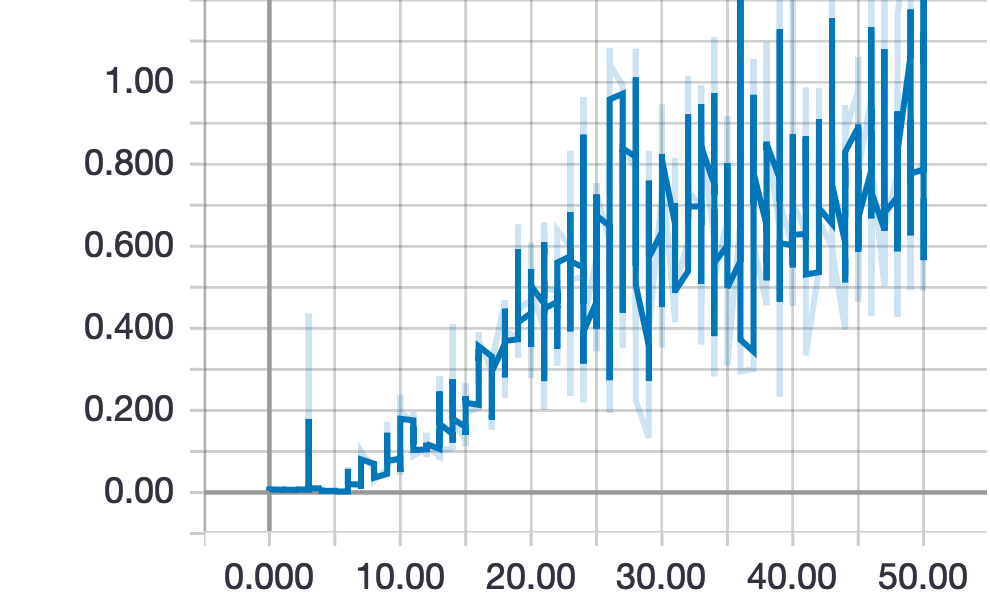
\includegraphics[width=0.3\textwidth]{arim/gan_training/anogan_loss_generator}} 
		& \subfloat[BiGAN generator
		training]{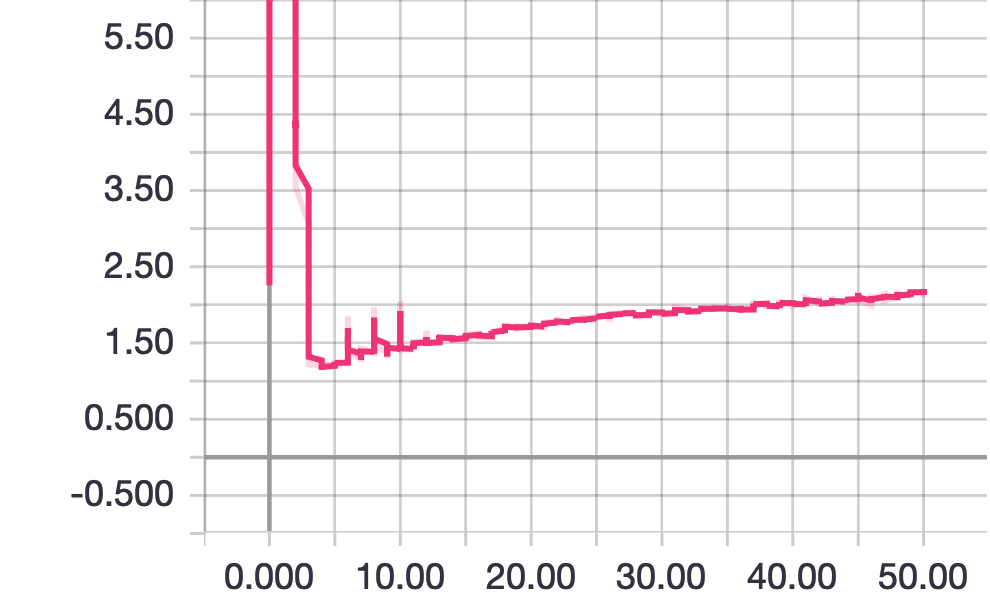
\includegraphics[width=0.3\textwidth]{arim/gan_training/bigan_loss_generator}} &
		\subfloat[ALAD generator
		training]{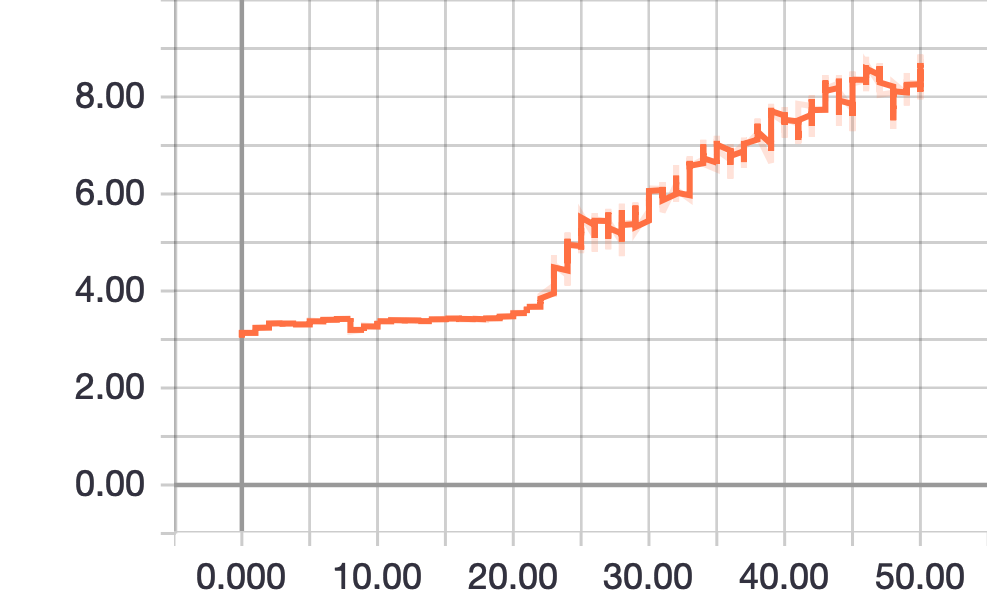
\includegraphics[width=0.3\textwidth]{arim/gan_training/alad_loss_generator}} \\
		\subfloat[AnoGAN discriminator training]{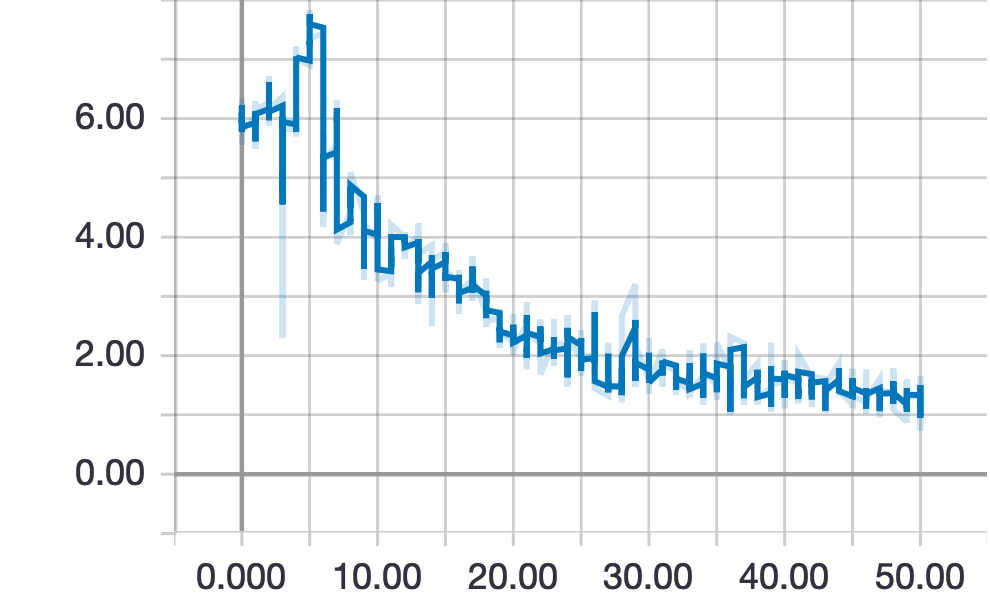
\includegraphics[width=0.3\textwidth]{arim/gan_training/anogan_loss_discriminator}} 
		& \subfloat[BiGAN discriminator
		training]{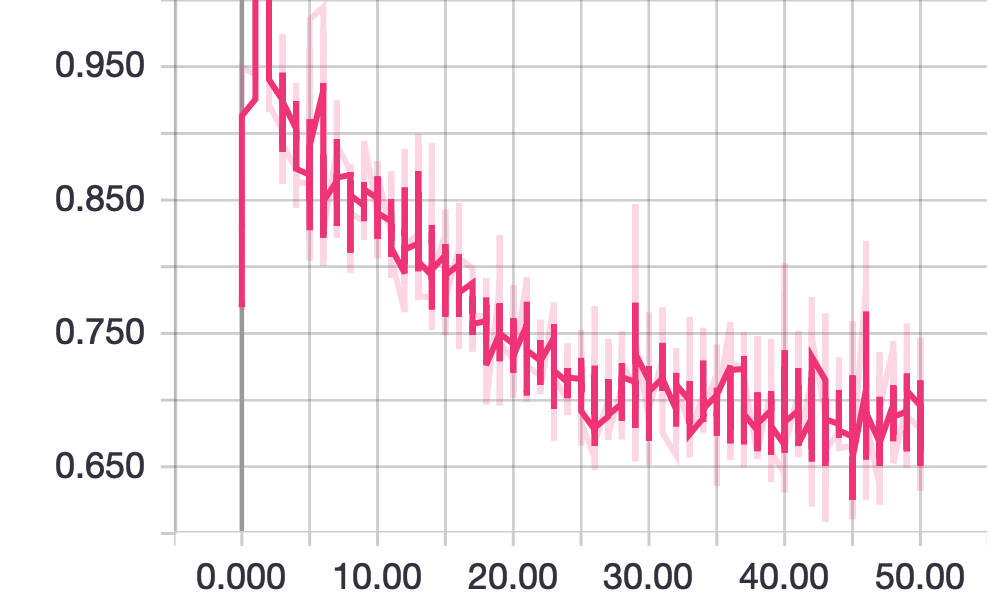
\includegraphics[width=0.3\textwidth]{arim/gan_training/bigan_loss_discriminator}}
		& \subfloat[ALAD discriminator
		training]{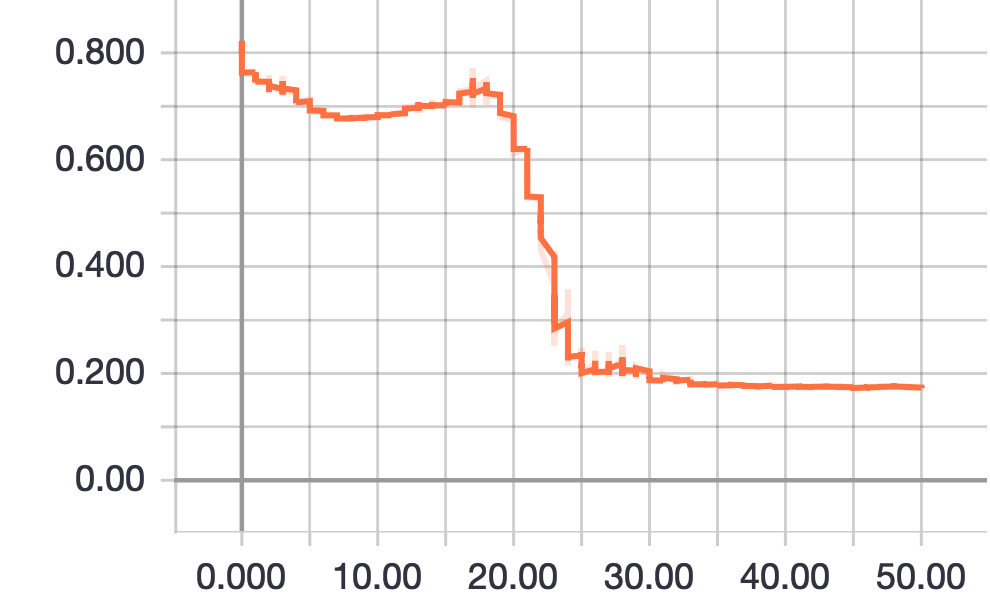
\includegraphics[width=0.3\textwidth]{arim/gan_training/alad_loss_discriminator}}
		\\
		\subfloat[AnoGAN generated image sample]{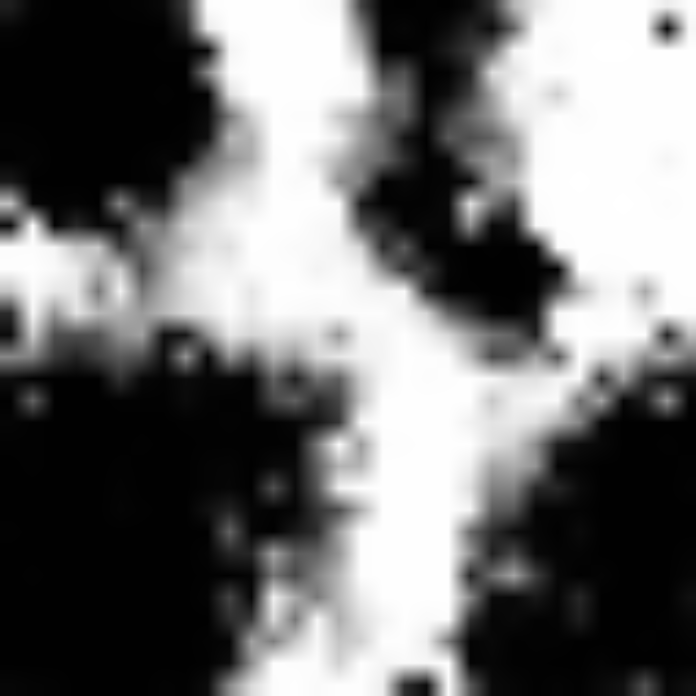
\includegraphics[width=0.3\textwidth]{arim/gan_training/anogan_gan}} 
		& \subfloat[BiGAN generated image
		sample]{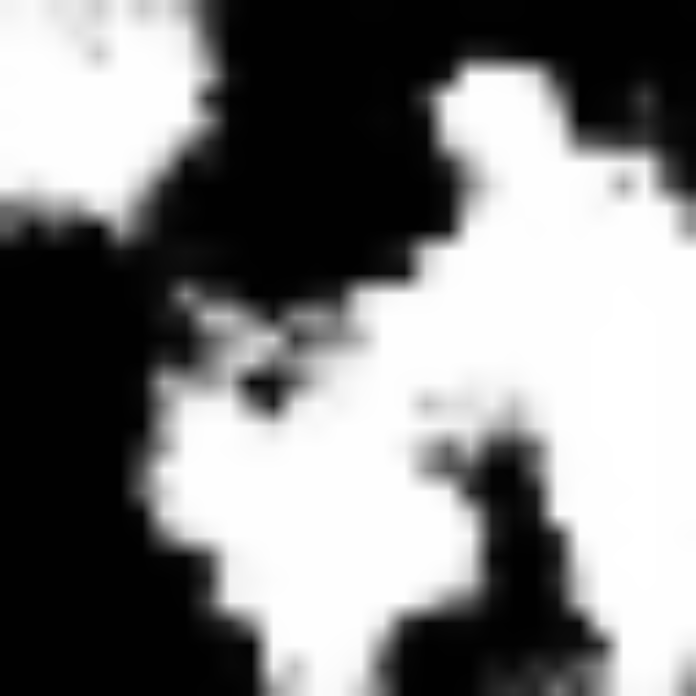
\includegraphics[width=0.3\textwidth]{arim/gan_training/bigan_gan}} & \subfloat[ALAD
		generated image sample]{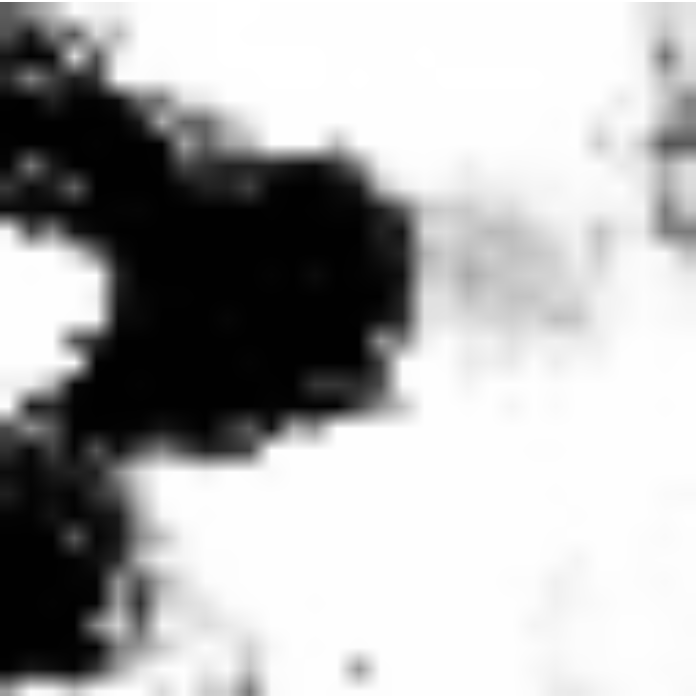
\includegraphics[width=0.3\textwidth]{arim/gan_training/alad_gan}}
	\end{tabular}
	\end{tabularx}
	\caption{Training information for the Pure GAN models. For graphs, x axis is the number of epochs and the y axis is the loss value}\label{fig:arim_training}
\end{figure}
%%%
As seen in the Figure \ref{fig:arim_training}, discriminator is gradually learning to differentiate between the real and
generated image while the generator network does not seem to set its loss to a certain level as
desired. This trend is observed in the majority of the experiments and in the ablation study as
well. From the perspective of the image generation, samples generated from GANs are not contextually
sound enough to represent the target distribution of the SEM image dataset. To obtain a more concise
observation the reconstructions from these GANs are also inspected (see Chapter \ref{chap:expres}). 

\begin{equation}
\label{eqn:ebgan_used}
\begin{aligned}
D(x)&=\|\operatorname{Dec}(E n c(x))-x\|\\[5pt]
V(G, D) &= D(G(z)) + D(x)+[m-D(G(z))]^{+} \\[5pt]
\mathcal{L}_{D}(x, z) &=D(x)+[m-D(G(z))]^{+} \\[5pt]
\mathcal{L}_{G}(z) &=D(G(z))
\end{aligned}
\end{equation}

Considering the results of these experiments and reconstruction samples of EBGAN (see Figure \ref{fig:ebgan_reconstruct}), training objective of the EBGAN model is adopted to
obtain a more stable training with our dataset which is presented in Equation \ref{eqn:ebgan_used} where 
$\mathcal{L}_{D}(x, z)$ is the training objective for discriminator network and $\mathcal{L}_{G}(z)$ is the 
training objective for the generator network.

Defining loss function as a value of energy still preserves the adversarial aspect of the objective
function. An autoencoder network acts as a discriminator network and attains energy values to the real
and fake image samples with high energy values assigned to generated images. Generator network tries to
"fool" the discriminator to decrease the amount of energy fake image is assigned. In this context, the energy
term is described as the ability of discriminator to reconstruct the given input, so it is a
reconstruction error based value. 

Using energy based GAN proved useful to obtain a consistent performance without having issues with
argued stabilization problems. Details regards to its training and model's reconstruction capability
will be discussed in its own section (see Section \ref{sec:exp_sencebgan}).

\subsection{Convergence of Encoder Training}
\label{sec:conv_enc}

Stabilizing the encoder network is actually the second step for a reconstruction based anomaly
detection approach. As proposed, generator network learns the mapping from the latent space $Z$ to
the image space $X$. However in order to test unknown images for anomalies, the latent
representation of the image must be extracted. From this point on this operation is called the
\textbf{inverse mapping}. Generators are not able to provide this kind of inverse mapping so pure GAN based
models followed different approaches to obtain this information.

AnoGAN model implements a back propagation routine for a predetermined number of steps to approximate
the latent representation of the query image. It randomly initializes a latent representation vector
and updates it until the loss that is defined as the $\ell_{2}$ norm of the query image and
generated sample converges. The main disadvantage of this approach is the time constraint. Method
works with image patches so processing whole image takes a considerable amount of time compared to
other methods.

BiGAN and ALAD integrates an additional encoder network to their adversarial training
to learn the inverse mapping while learning the image distribution (see Equation \ref{eqn:alad_bigan_eqn}).

\begin{equation}
\label{eqn:alad_bigan_eqn}
\begin{aligned} V\left(D, E, G\right) &=\mathbb{E}_{x \sim p_{\text{data}}}\left[\log D_{x z}(x, E(x))\right] \\ &+\mathbb{E}_{z \sim p_{Z}}\left[1-\log D_{x z}(G(z), z)\right]
\end{aligned}
\end{equation}

To learn both mappings, models learn the joint probability distribution of the image and the noise
pairs. Discriminator network therefore is modified to process this new representation (see
implementation details in Appendix Section \ref{app:bigan} and \ref{app:alad}). Integrating an encoder
network solves the time constraint problem because the latent representation is acquired with
feeding the query image to the encoder network at the inference stage and the computation time is
negligible compared to AnoGAN's approximation method. Nonetheless addition of a new component to the
adversarial training brings new stabilization problems with regards to encoder network. Training of
the generator discriminator, implicitly affects the quality of the representation encoded by the 
encoder network. ALAD implements additional discriminators to control the conditional probability 
distributions of the learned joint distribution from both ends (For noise and for image) to improve 
the encoder performance but experiments did not provide a considerable advancement even with ablation 
study. Figure \ref{fig:arim_encoder} presents the training graphs of the models and their obtained
reconstructions. AnoGAN model does not have a training graph for encoder since it uses a
back propagation and it would have a convergence graph for each patch in the dataset. Instead, the
training graph of the first iteration of the proposed model's (see Section \ref{sec:encebgan}) 
encoder is presented for comparison. 
\begin{figure}[h!]
	\def\tabularxcolumn#1{m{#1}}
	\begin{tabularx}{\linewidth}{@{}XXX@{}}
		\begin{tabular}{ccc}
			\subfloat[BiGAN Encoder Training]{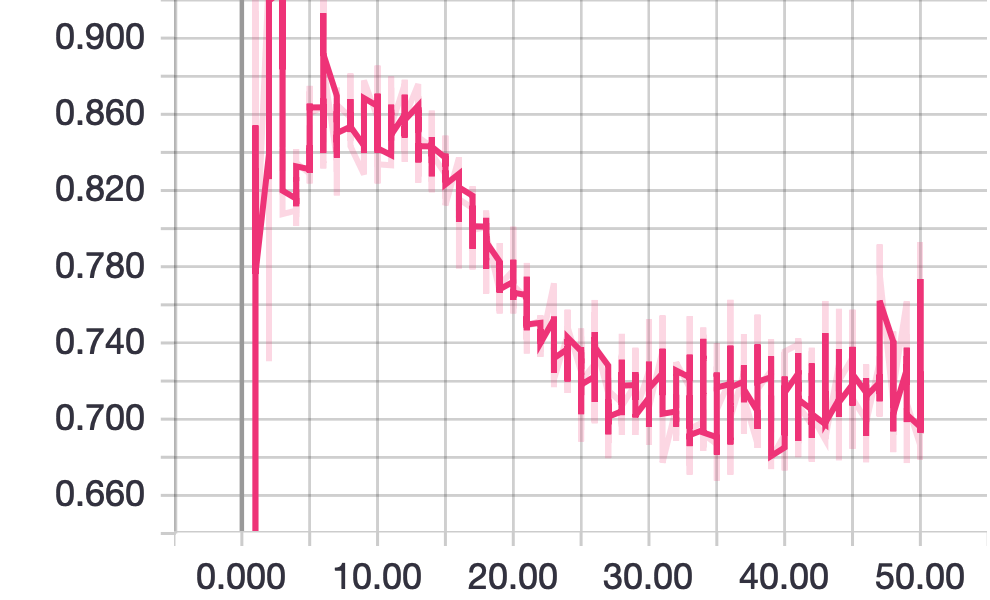
\includegraphics[width=0.3\textwidth]{arim/encoder_conv/bigan_loss_encoder}} 
			& \subfloat[ALAD Encoder
			Training]{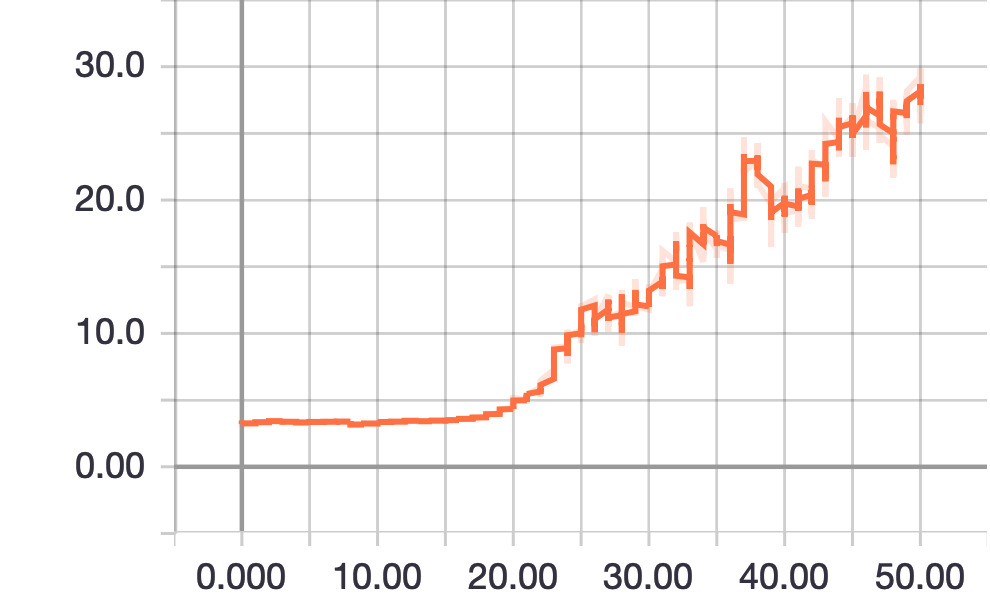
\includegraphics[width=0.3\textwidth]{arim/encoder_conv/alad_loss_encoder}} &
			\subfloat[ENCEBGAN Encoder
			Training]{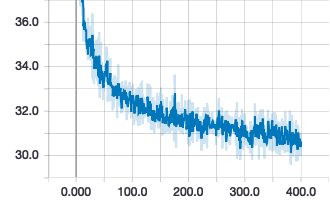
\includegraphics[width=0.3\textwidth]{arim/encoder_conv/enceb_loss_encoder}}
			
		\end{tabular}
	\end{tabularx}
	\caption{Training graphs of pure GAN models that implement encoder network and the first iteration of the proposed network}\label{fig:arim_encoder}
\end{figure}

By itself, these training graphs does not give us a reliable insight about encoder performance.
Other than its quantitative results, encoder networks performance can be quantified with models'
ability to reconstruct a given image after training. At this point in pipeline, impact of a good
generator also comes into play. In both models, training of the encoder network is computed by
feeding the latent representation obtained from the encoder  to the generator to
reconstruct the training data. So performance and proper training of the encoder network also
depends on the adversarial training of generator network. In the mini max game played by BiGAN and ALAD, both
encoder and generator networks tries to fool the discriminator. Therefore stabilization problem of generator
inadvertently affects the encoder convergence which also affects the quality of the reconstructions
obtained from the model. Some distortions and the information loss is expected in the generator
based reconstruction. In our dataset, these imperfections cause reconstructed samples to be
interpreted as anomalous sample though the input is a normal sample. Figure
\ref{fig:arim_reconstruct} shows the reconstructions from AnoGAN, BiGAN and ALAD's inference stage. 

\begin{figure}[!ht]	
	\def\tabularxcolumn#1{m{#1}}
	\begin{tabularx}{\linewidth}{@{}XXX@{}}
		\begin{tabular}{ccc}
			\subfloat[AnoGAN Query Image]{
\includegraphics[width=0.3\textwidth]{arim/encoder_conv/anogan_sample}} 
			& \subfloat[BiGAN Query
			Image]{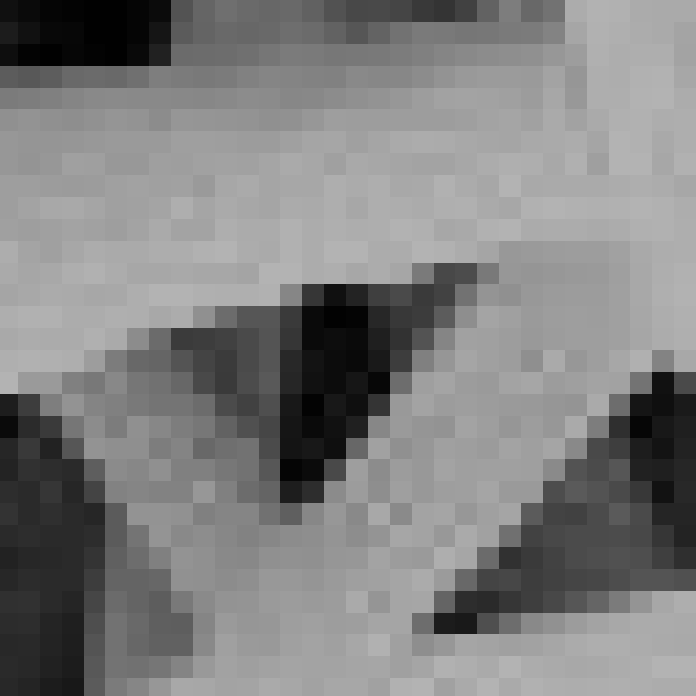
\includegraphics[width=0.3\textwidth]{arim/encoder_conv/bigan_sample}} &
			\subfloat[ALAD Query
			Image]{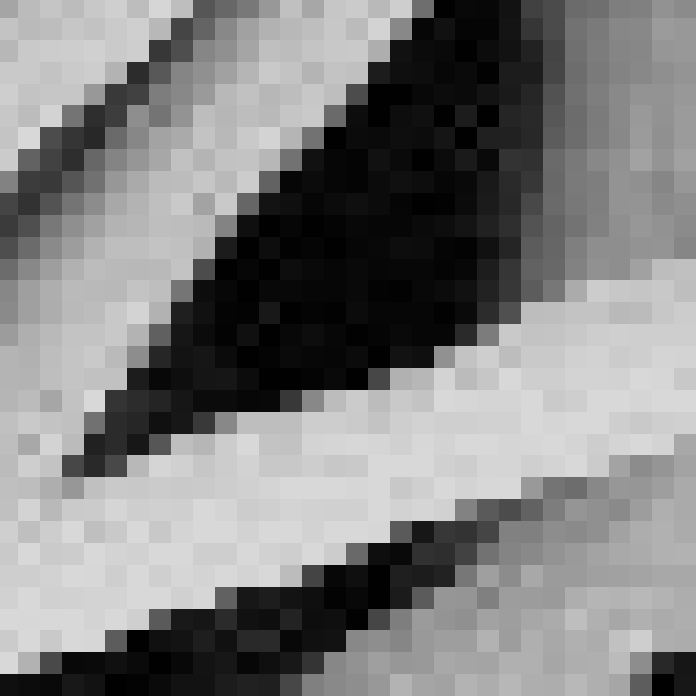
\includegraphics[width=0.3\textwidth]{arim/encoder_conv/alad_sample}} \\
			\subfloat[AnoGAN Reconstruction]{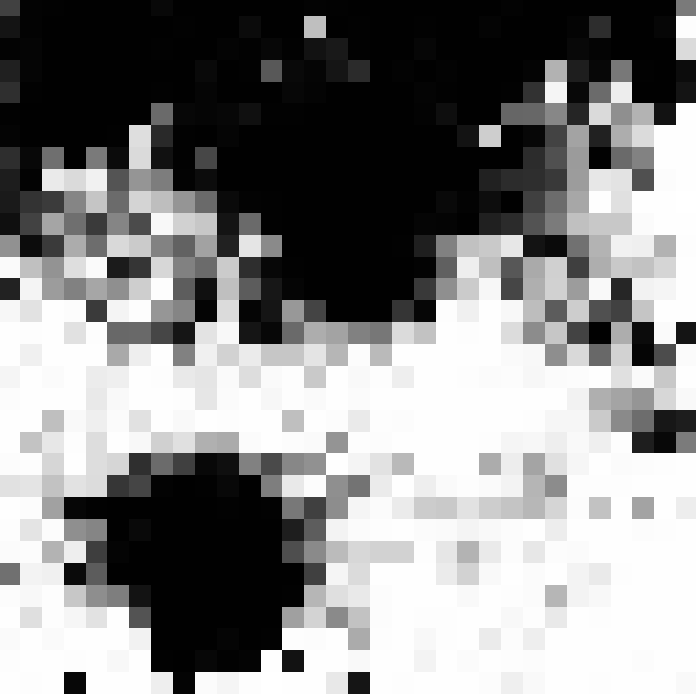
\includegraphics[width=0.3\textwidth]{arim/encoder_conv/anogan_reconstruct}} 
			& \subfloat[BiGAN
			Reconstruction]{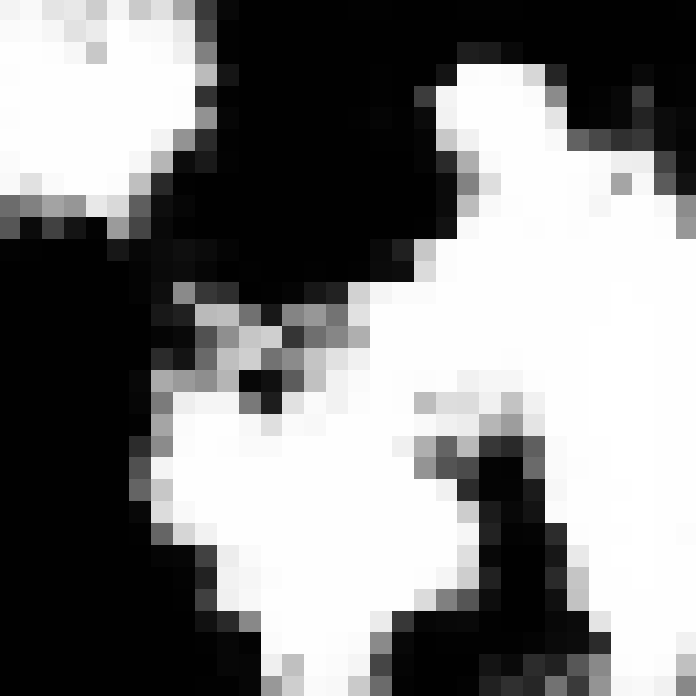
\includegraphics[width=0.3\textwidth]{arim/encoder_conv/bigan_reconstruct}}
			& \subfloat[ALAD
			Reconstruction]{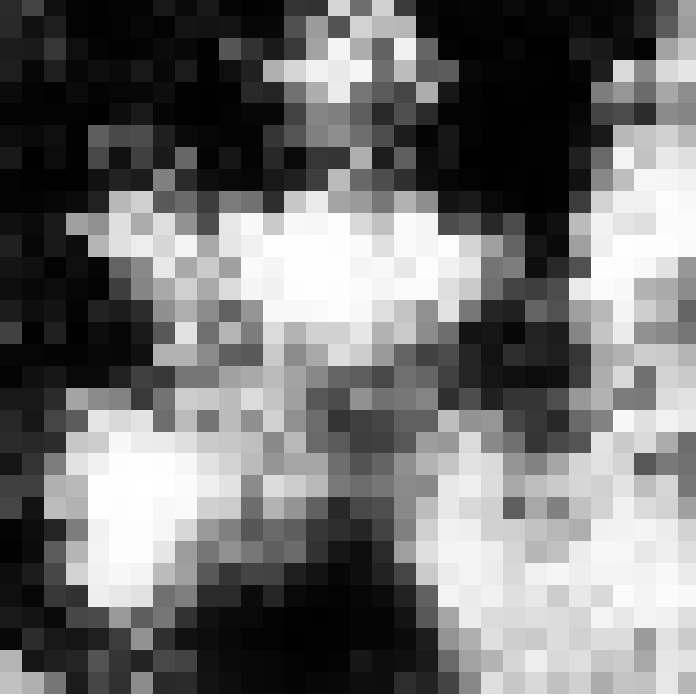
\includegraphics[width=0.3\textwidth]{arim/encoder_conv/alad_reconstruct}}
			
		\end{tabular}
	\end{tabularx}
	\caption{Reconstructed samples from the pure GAN models. Upper row is the given query image and the bottom row is their reconstructions}\label{fig:arim_reconstruct}
\end{figure}

Proposed model in this thesis also uses additional encoder network to get the inverse mapping
of image and latent representation space. Several modifications are applied to the training in order to improve the stabilization
and ensure the convergence of the encoder network. Equation \ref{eqn:ebgan_used} propose the modified generator
discriminator network approach. Addition of the encoder network and its training is also based on the reconstruction 
energy defined in Section \ref{sec:ebgan}.
\begin{equation}
\label{eqn:encebgan_used}
\begin{aligned}
D(x)&=\|\operatorname{Dec}(E n c(x))-x\|\\[5pt]
V(G,E, D) &= D(G(z)) + D(x)+[m-D(G(z))]^{+} + D(G(E(x))) \\[5pt]
\mathcal{L}_{E}(x) &= D(G(E(x)))
\end{aligned}
\end{equation}

Like AnoGAN and ALAD, proposed model also trains encoder network with generator networks help to
obtain the reconstruction. However, instead of training all the networks in the adversarial setting,
proposed model separates the training of the generator discriminator pair and the encoder network.
Training strategy presented in F-AnoGAN framework (see Section \ref{sec:fanogan}) proposes an
initial adversarial training. In the second part of the training the encoder network is trained by
creating a pipeline with the other network components with fixed weights (inference mode) (See
Figure \ref{fig:fanogan_training}). This approach focuses on the encoder training objective by
removing the dependency between encoder and generator networks which in turn also decreases the potential
convergence issues of the encoder network.

So far, configuring the models' objective function to an energy based setting and separating the
joint training into sequential steps give the model two opportunities:

\begin{itemize}
	\item {The stabilization of the GAN training, which means better reconstruction performance.}
	\item {Easy convergence for encoder network because it isn't trained concurrently with the
	generator so learning latent reprensetation does not depend of the learning progress of the generator network. }
\end{itemize}

Net section will discuss our proposed model with the mentioned changes and continue to analyze the
existent shortcomings despite these applied improvements.


\section{Encoded Energy Based Generative Adversarial Network}
\label{sec:encebgan}

First iteration of the proposed model is called encoded energy based generative adversarial
network,or ENCEBGAN. This section presents how its built, its training scheme and the issues it
solved.

ENCEBGAN consists of an energy based generative adversarial network framework with an additional
encoder network. Roles of the corresponding networks are identical to BiGAN (see Section \ref{sec:bigan}). Two main
differences are the change in the rationale in adversarial training component and separation of the
encoder network training. Figure \ref{fig:encebgan_model} presents the model components with an
emphasis on the training sequence.
\begin{figure}[h!]
	\centering
	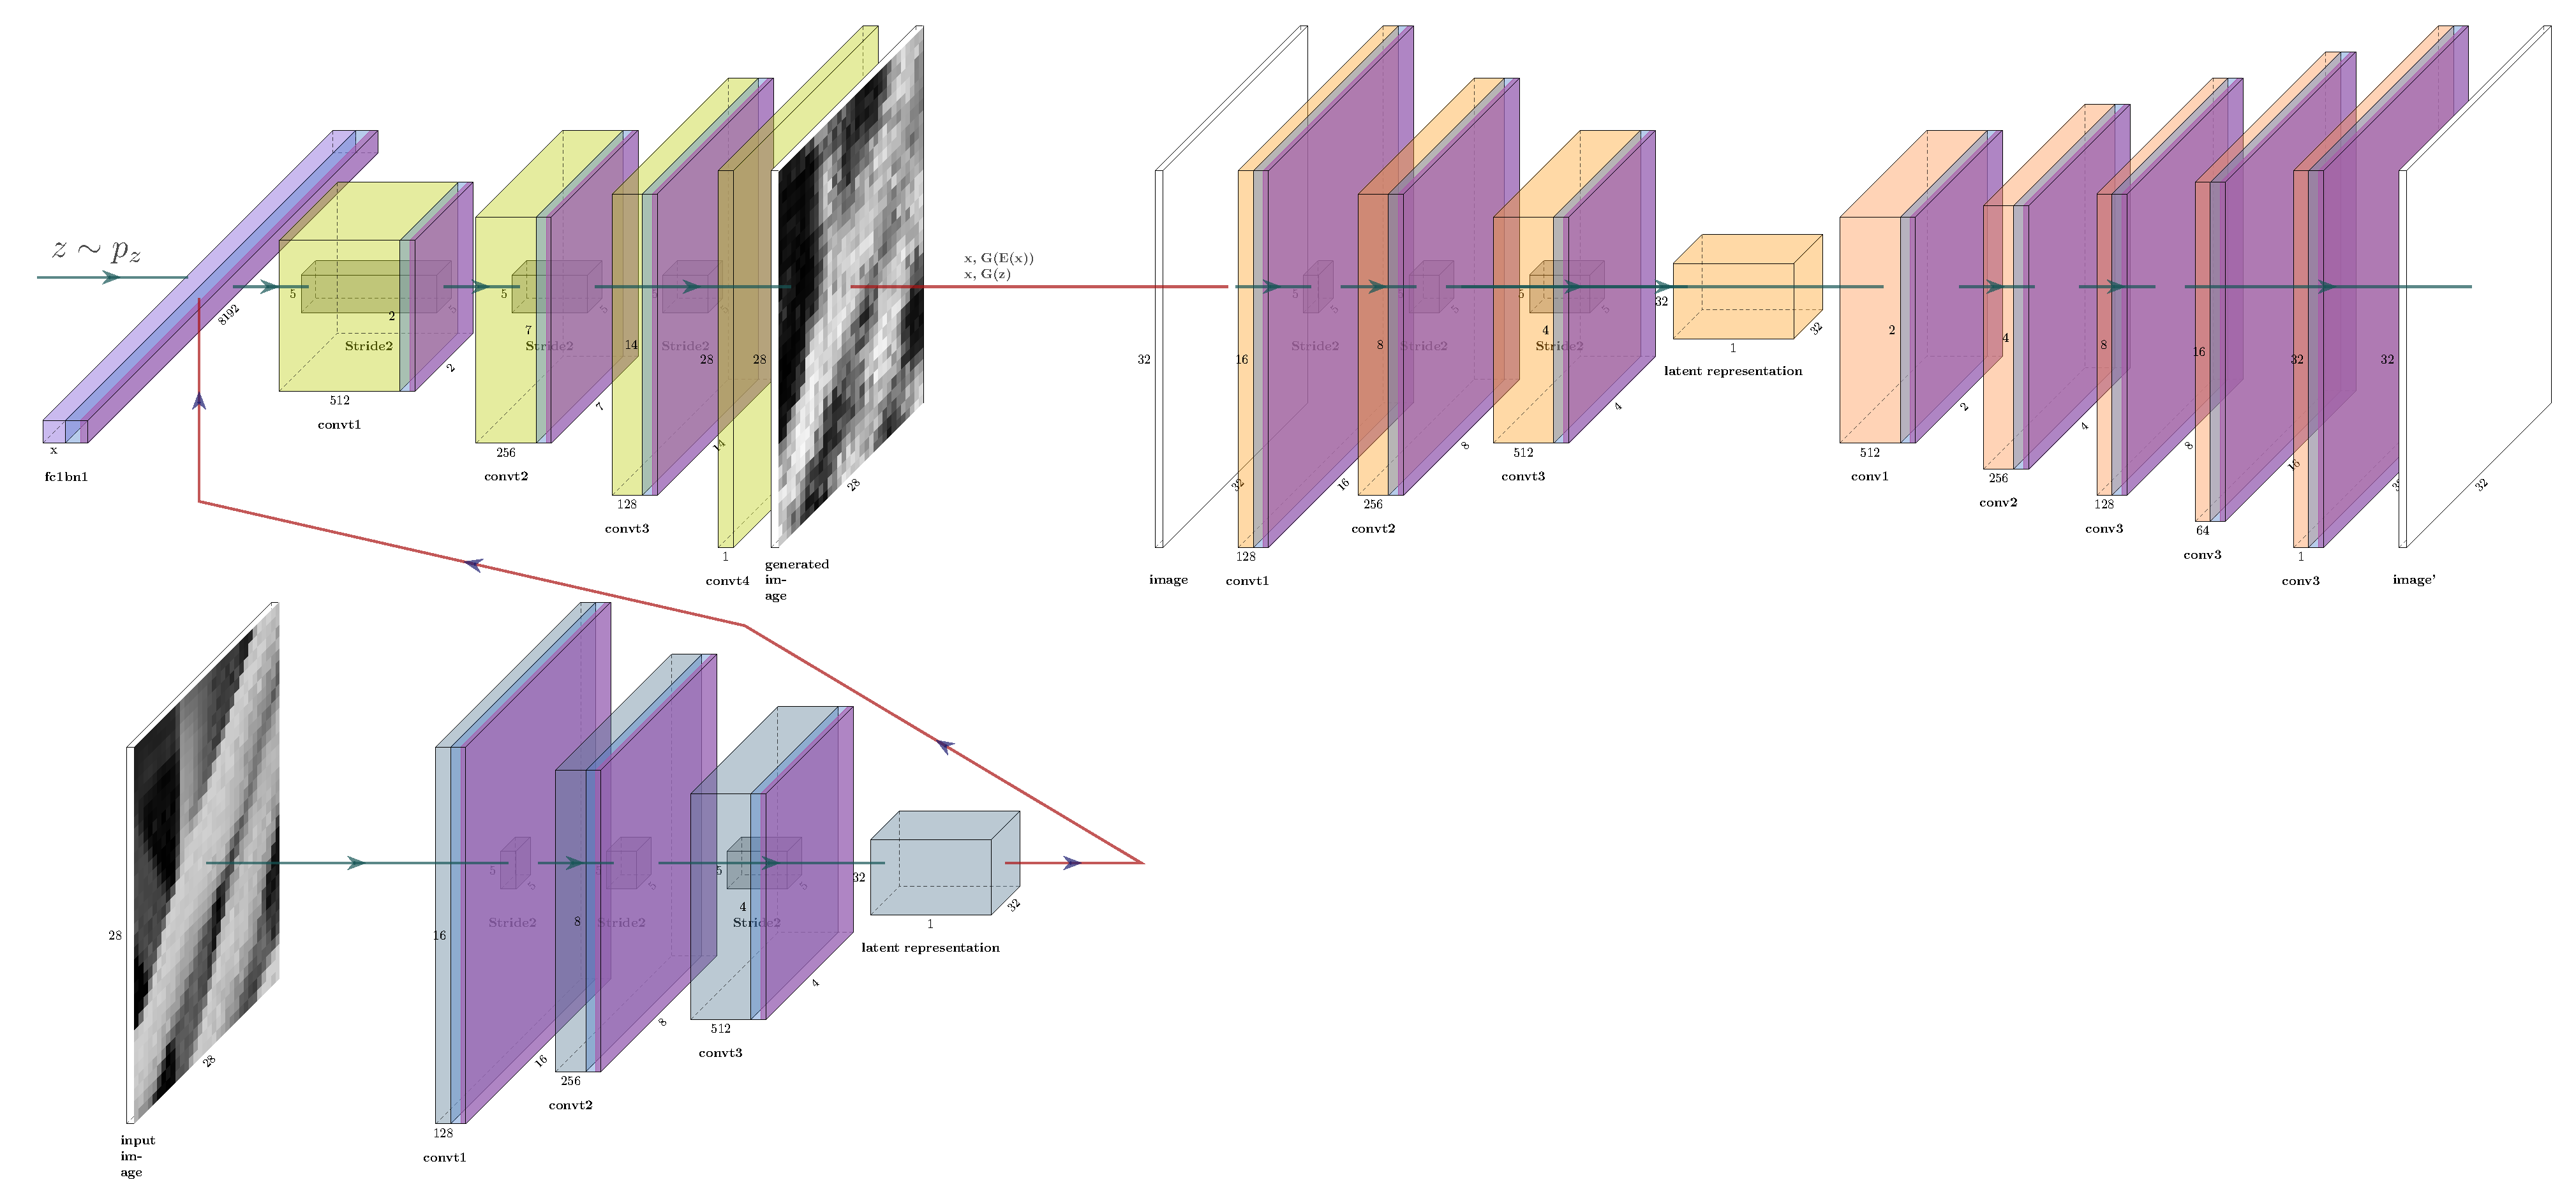
\includegraphics[width=1.0\textwidth]{arim/encebgan/encebgan}
	\caption{ENCEBGAN Model Overview }
	\label{fig:encebgan_model}
\end{figure}

Training of the model is divided into two sections. In the first section generator and discriminator networks
train adversarially to learn the mapping from image space to latent space. While generator learns
the mapping, discriminator is concurrently learning to reconstruct the training dataset and learns
to encode the training data on its own. This latent representation will be used later on as an
auxiliary information for anomaly score computation. After the adversarial training is completed,
pipeline is created from the encoder generator networks to form a conceptual autoencoder and whole
network is trained using the reconstruction error based objective function for the encoder network (see Equation \ref{eqn:fanogan_rec_loss}).
In second stage, generator and discriminator don't learn any additional information about the
dataset. This approach proved to be useful to stabilize both generator and encoder hence increased
the reconstruction quality of our model. Anomaly score computation is the same as the pure GAN based
methods which is the reconstruction error between the query and the output of encoder generator
pipeline as depicted in Equation \ref{eqn:enceb_ad}. 
\begin{equation}
	\label{eqn:enceb_ad}
	\mathcal{A}(x) = \norm{x - G(E(x))}^2
\end{equation}

Figure \ref{fig:arim_encebgan_info} presents the training graph information and reconstructed
samples as a comparison to reconstructions in Figure \ref{fig:arim_reconstruct}.
\begin{figure}[!ht]	
	\def\tabularxcolumn#1{m{#1}}
	\begin{tabularx}{\linewidth}{@{}XXX@{}}
		\begin{tabular}{ccc}
			\subfloat[Generator Training Graph]{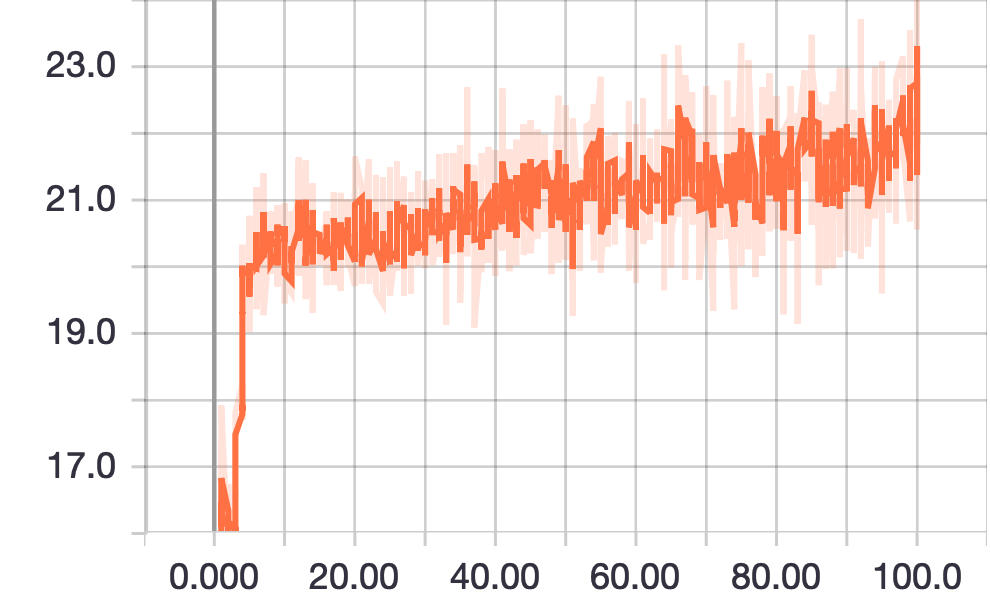
\includegraphics[width=0.3\textwidth]{arim/encebgan/encebgan_loss_generator}} 
			& \subfloat[Discriminator Training
			Graph]{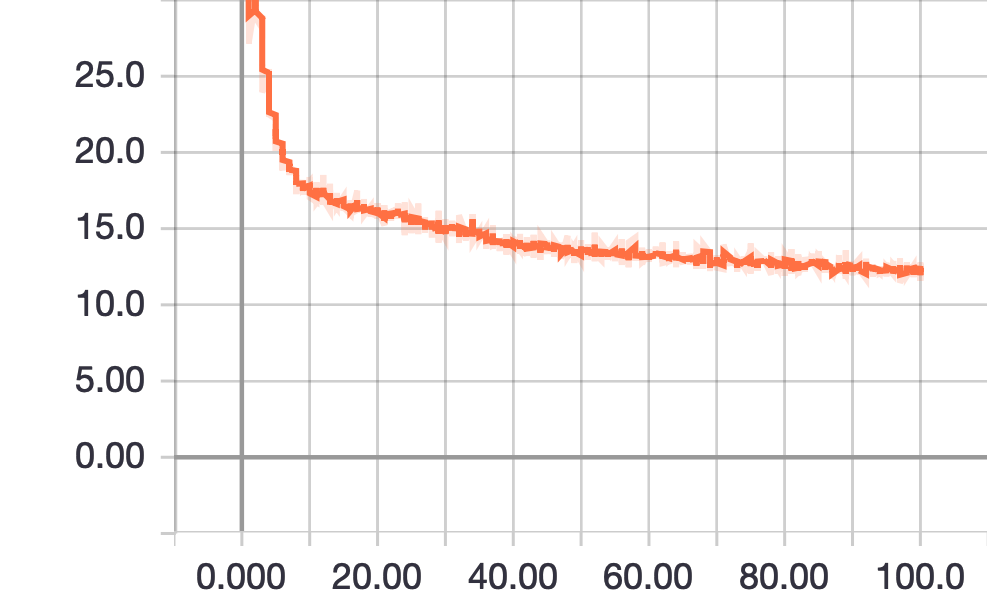
\includegraphics[width=0.3\textwidth]{arim/encebgan/encebgan_loss_discriminator}}
			& \subfloat[Encoder Training
			Graph]{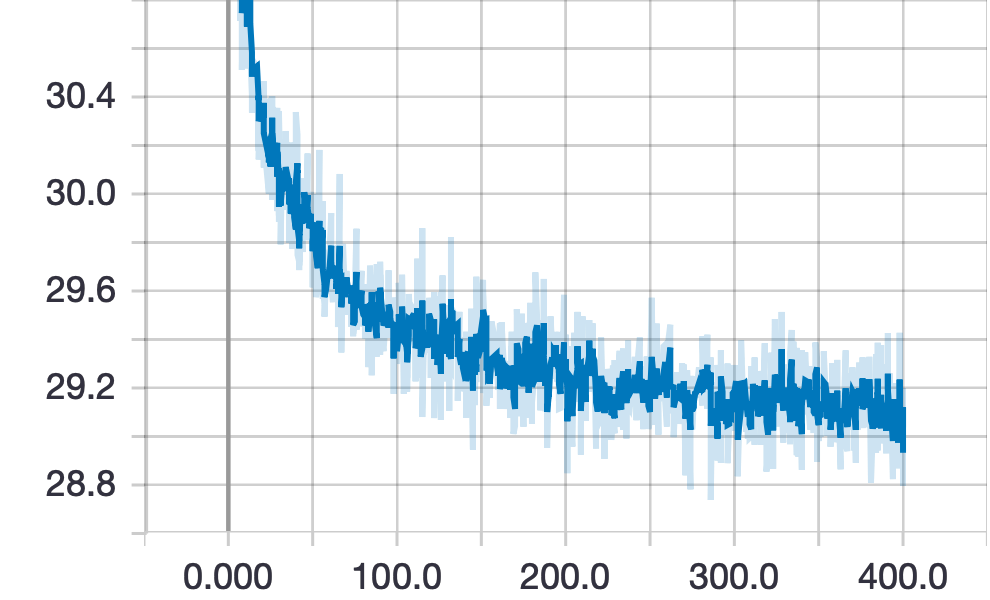
\includegraphics[width=0.3\textwidth]{arim/encebgan/encebgan_loss_encoder}} \\
			\subfloat[ENCEBGAN Generated Sample]{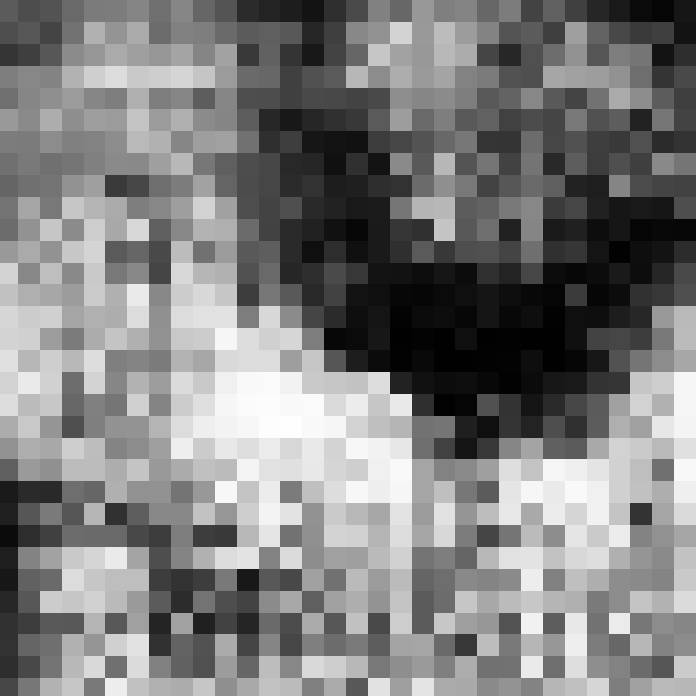
\includegraphics[width=0.3\textwidth]{arim/encebgan/encebgan_generated}} 
			& \subfloat[ENCEBGAN Query
			Sample]{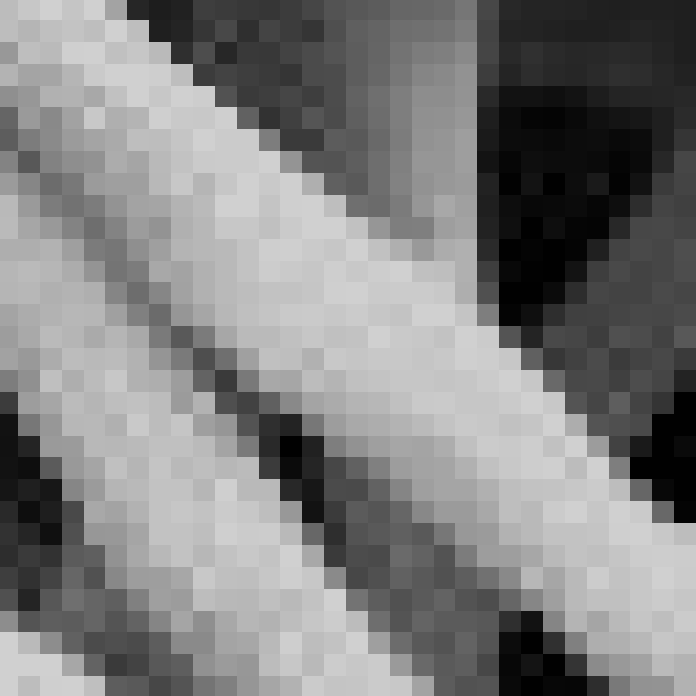
\includegraphics[width=0.3\textwidth]{arim/encebgan/encebgan_input}} &
			\subfloat[ENCEBGAN
			Reconstruction]{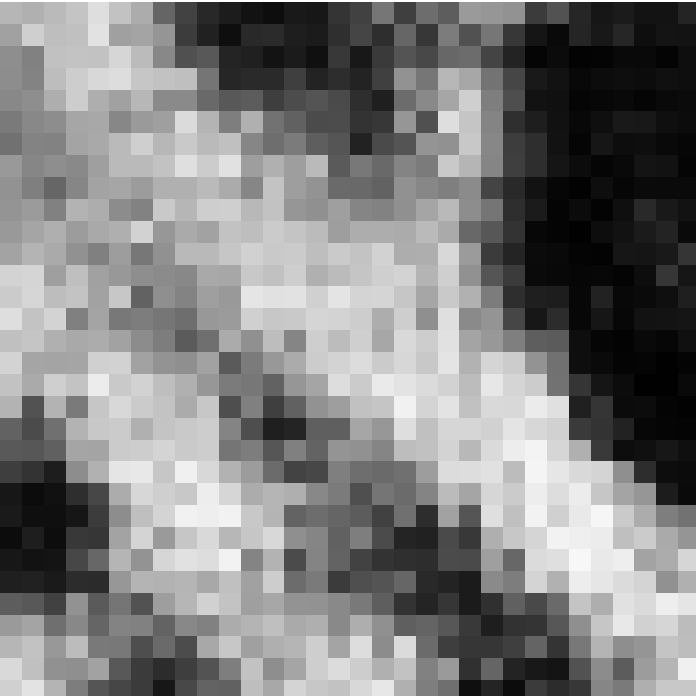
\includegraphics[width=0.3\textwidth]{arim/encebgan/encebgan_reconstruct}}\\
			
		\end{tabular}
	\end{tabularx}
	\caption{Training graphs and qualitative examples from ENCEBGAN Model}\label{fig:arim_encebgan_info}
\end{figure}

With previously mentioned architectural improvements, ENCEBGAN performed better than BiGAN and ALAD
and obtained a similar performance as AnoGAN which will discussed in Chapter \ref{chap:expres}.
Separating the training of encoder and changing the adversarial objective function mechanics
consequently stabilized the convergence of both networks and the reconstruction quality has
increased compared to the pure GAN based models.

Imperfections in the reconstructions are usually expected in reconstruction based anomaly detection
methods since the network trained to learn the latent representation is regularized to prevent
overfitting. In SEM image dataset, anomalous regions can occur in any level of the image with
varying levels of brightness. During the experiments of the models it is observed that,
imperfections in the reconstructions may be identified as anomalous regions even though the image is
anomaly free. This issue inadvertently cripples the anomaly detection performance of ENCEBGAN (and
other pure GAN based models). 

Next section will discuss the anomaly score computation methods featured in both pure GAN based and
autoencoder variant models, and explain the addition of a secondary encoder network to improve the
overall performance of the proposed model.

\subsection{Anomaly Score Computation}
\label{sec:as_compute}

Previously we divided the state of the art GAN based anomaly detection methods into two main
categories. Pure GAN based models and autoencoder variants. The main difference between these groups
is that decoder (generator equivalent) network of these models is trained only with the latent
representation of the image supplied from the encoder network. Since they learn to reconstruct using
the encoded version of the training data, their reconstructions are superior compared to the pure
GAN based methods. Figure \ref{fig:arim_anoscore} shows an example reconstruction from both GANomaly
and Skip-GANomaly (see Section \ref{sec:ganomaly}). 

\begin{figure}[!ht]	
	\def\tabularxcolumn#1{m{#1}}
	\begin{tabularx}{\linewidth}{@{}XXX@{}}
		\begin{tabular}{ccc}
			\subfloat[Query Sample]{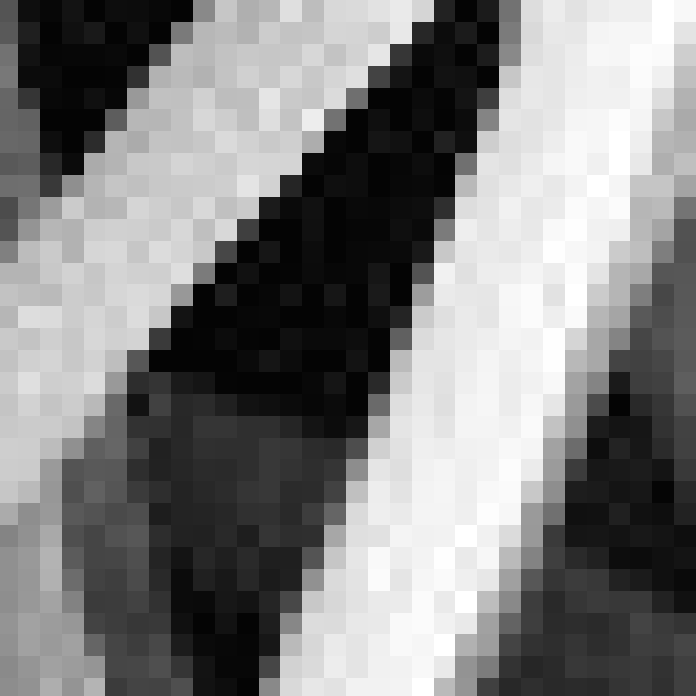
\includegraphics[width=0.3\textwidth]{arim/anomaly_score/anoscore_input}} 
			& \subfloat[GANomaly
			Reconstruction]{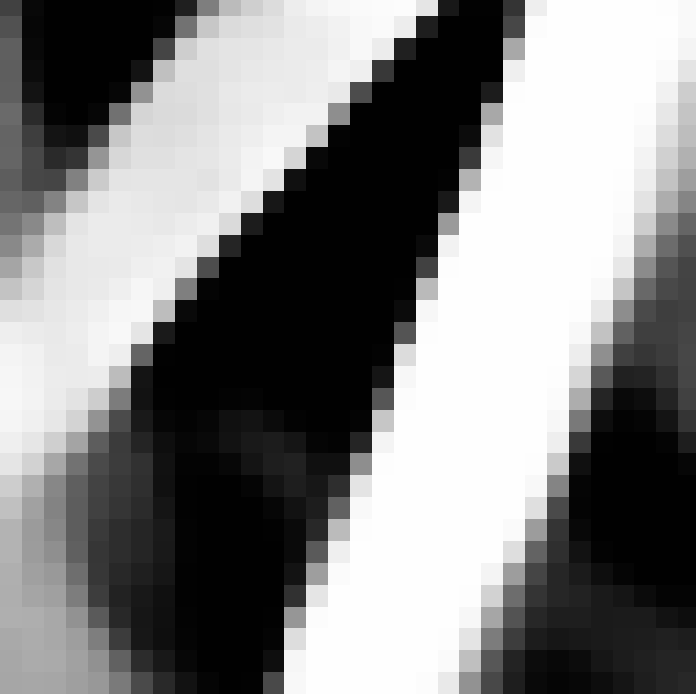
\includegraphics[width=0.3\textwidth]{arim/anomaly_score/anoscore_ganomaly}}
			& \subfloat[Skip-GANomaly
			Reconstruction]{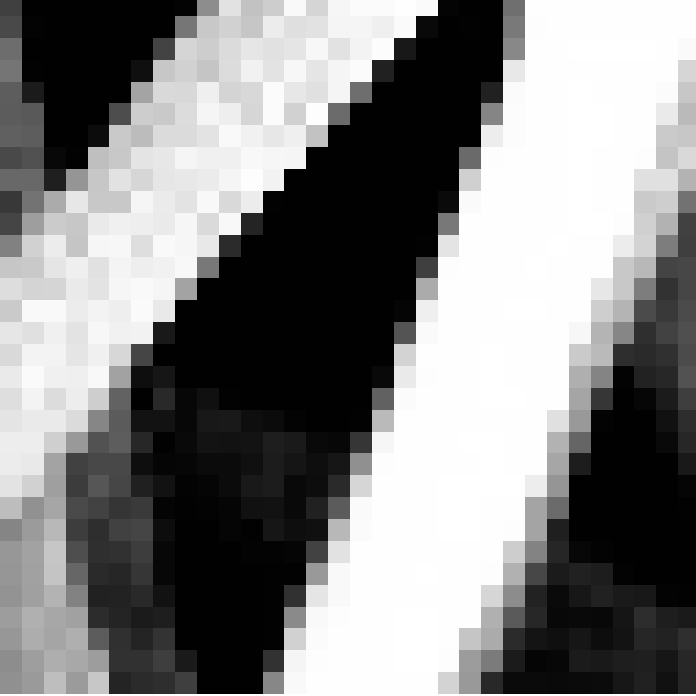
\includegraphics[width=0.3\textwidth]{arim/anomaly_score/anoscore_sganomaly}}
			\\			
		\end{tabular}
	\end{tabularx}
	\caption{Reconstruction examples of Autoencoder Variant Models}\label{fig:arim_anoscore}
\end{figure}

Architectural difference between GANomaly and Skip-GANomaly is the additional skip connections
between the encoder and decoder network of the latter. This information transfer enables
Skip-GANomaly to retain more information about the data and help it to accumulate this data across
the layers during the decoding stage of the reconstruction. One interesting observation is that even
though the general quality of the Skip-GANomaly model is better than GANomaly on the SEM image
dataset, ablation studies performed in Chapter \ref{chap:expres}(see Table \ref{tab:ganomaly_ablation}
and \ref{tab:sganomaly_ablation}) show that overall GANomaly prediction performance is superior
compared to Skip-GANomaly. 

Both anomaly score computation is based on the reconstruction based error, but GANomaly uses a
secondary encoder network to learn the latent representation of the reconstruction and uses this
information to compute the anomaly score (see Equation \ref{eqn:ganomaly_as}). Skip-GANomaly on the
other hand composes the contextual data (reconstruction loss) with the latent loss which is obtained
from the feature layer of its discriminator network (see Equation \ref{eqn:sganomaly_as}). We hypothesize
that training a secondary encoder network improved GANomaly model's interpretation of the anomalous
sample data. Erroneous predictions that are caused due to misinterpreting imperfect reconstructions
as samples that contains anomalous regions may be averted by interpreting both input image and its
reconstruction at the latent dimensional complexity. 

Considering these observations and related improvements, Section \ref{sec:sencebgan} will present the final version
of the proposed model for anomaly detection. General architecture of the model, its training
procedure and its inference stage for anomaly detection will be discussed.


\section{Sequentially Encoded Energy Based Generative Adversarial Network}
\label{sec:sencebgan}

Sequentially encoded energy based generative adversarial network is the main proposed model that
aims to mitigate the disadvantageous outcomes of stabilization and convergence problems experienced
by the previously mentioned methods (see Chapter \ref{chap:sota}). Even though it is presented
incrementally throughout the chapter, its general architecture, training strategy and its approach
to anomaly detection problem will be discussed.
\begin{figure}[h!]
	\centering
	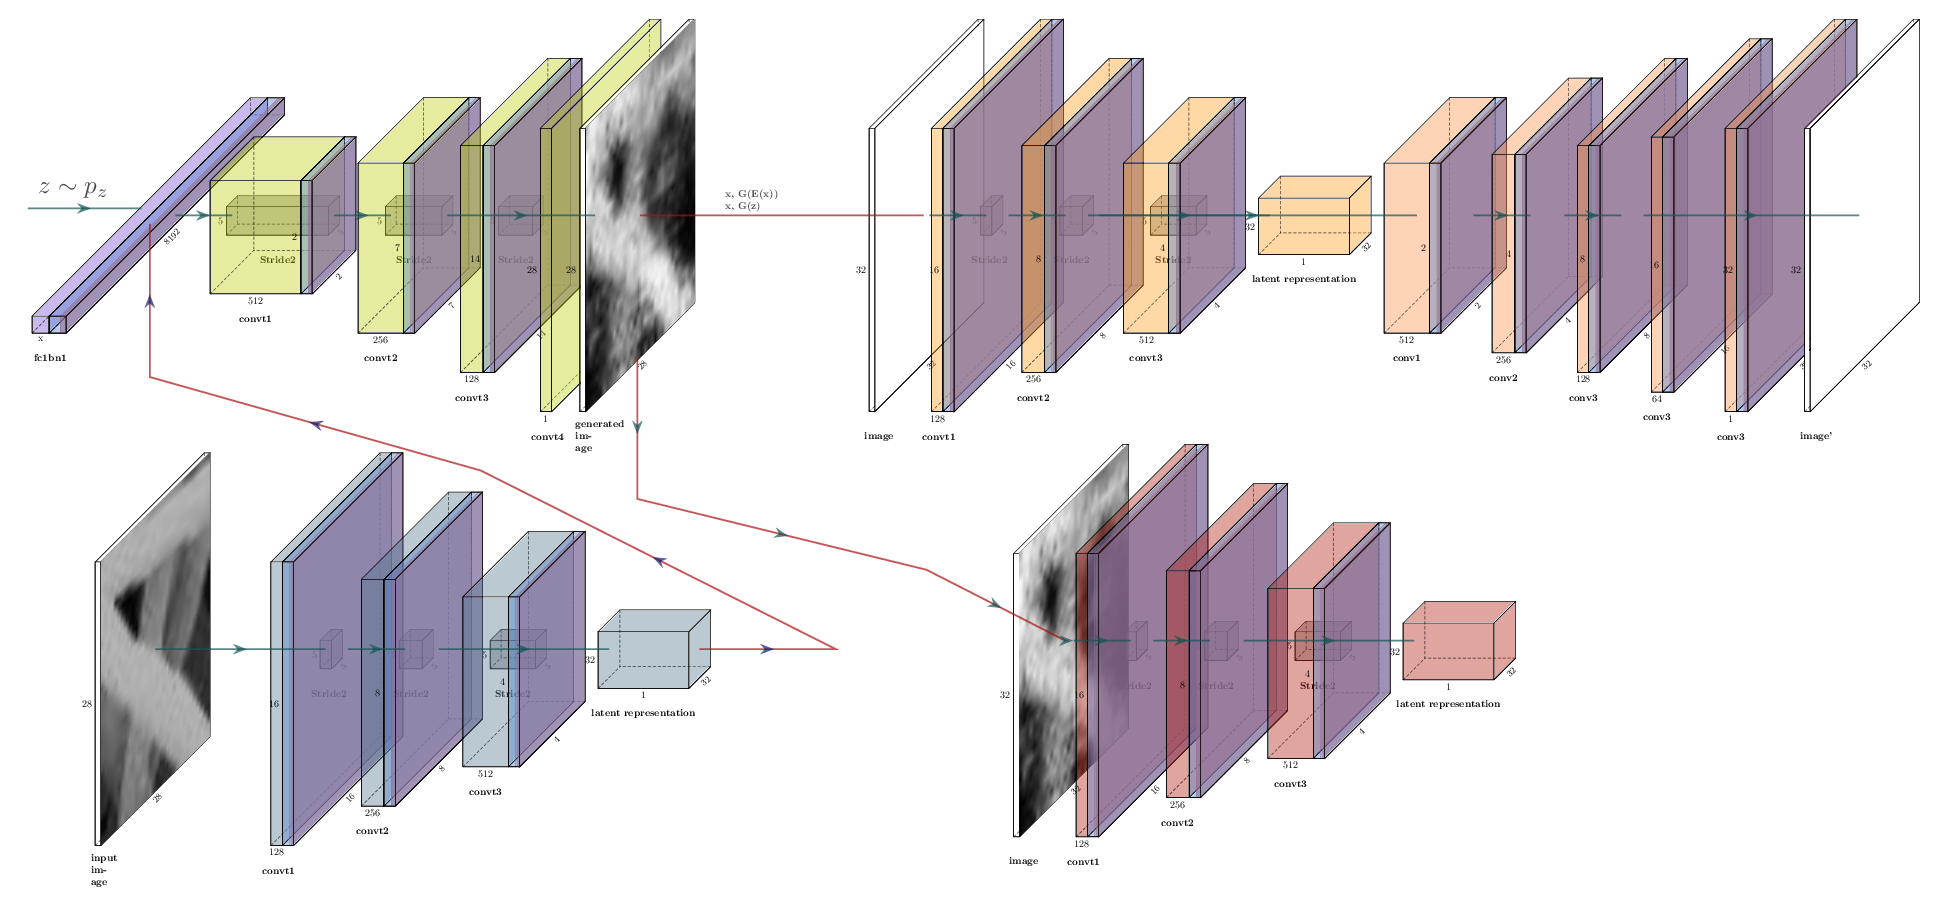
\includegraphics[width=1.0\textwidth]{arim/sencebgan/sencebgan}
	\caption{SENCEBGAN Model Overview }
	\label{fig:sencebgan_model}
\end{figure}

SENCEBGAN model consists of an energy based generative adversarial network and 2 additional encoder
networks. First encoder network learns the representation of training data and its called
generator encoder or $E_{G}$. Second encoder network learns the latent representation of the reconstructions
of the training data provided by the generator network. This encoder network will be mentioned as
reconstruction encoder or $E_{R}$. Training objective of the model is given in Equation
\ref{eqn:sencebgan_formula}.
\begin{equation}
	\begin{aligned}
		D(x)&=\|\operatorname{Dec}(E n c(x))-x\|\\[5pt]
		V(G,E_{G},E_{R}, D) &= \underbrace{D(G(z))}_{\text{Generator}} + \underbrace{D(x)+[m-D(G(z))]^{+}}_{\text{Discriminator}} +\\ & \underbrace{D(G(E_{G}(x)))}_{\text{Encoder}_{G}} + \underbrace{\norm{E_{G}(x) - E_{R}(G(E_{G}(x)))}^2}_{\text{Encoder}_{R}}
	\end{aligned}
	\label{eqn:sencebgan_formula}
\end{equation}

Training objective is divided into three separate sequences. In the first stage of the training,
energy based gan model (generator and discriminator networks) is trained. After the training 
is completed, autoencoder network is formed by merging $E_{G}$ and Generator network $G$ with fixed weights. 
Combined with discriminator (also fixed weights) $E_{G}$ is trained using the reconstruction 
error produced from the temporary autoencoder configuration. In the last stage, $E_{R}$ is 
trained to learn the latent representation of the reconstructed samples. Training is performed 
using the $\ell_{2}$ norm of the encoded representation residual (see Equation \ref{eqn:sencebgan_loss}). 
\begin{equation}
	\label{eqn:sencebgan_loss}
	\begin{aligned}
		\mathcal{L}_{E_{G}}(x) &= D(G(E(x))) \\[5pt]
		\mathcal{L}_{E_{R}}(x) &= \norm{E_{G}(x) - E_{R}(G(E_{G}))(x)}^2
 	\end{aligned}
\end{equation}

SENCEBGAN model separates anomaly detection computation into image based and latent dimension based
categories. Different anomaly score computations are tested to measure the impact of the additional
encoder networks and observe both implicit encoding and reconstruction capability of the
discriminator network. 
\begin{equation}
	\label{eqn:sencebgan_eqn_im}
	\begin{aligned}
	\mathcal{A}_{R}(x) & = \norm{x - G(E_{G}(x))}^ 2 \\[5pt]
	\mathcal{A}_{R_{D}}(x) & = \norm{D(x) - D(G(E_{G}(x)))}^2\\[5pt]
	\mathcal{A}_{IC}(x) & = \lambda \cdot \mathcal{A}_{R}(x) + (1 - \lambda) \cdot \mathcal{A}_{R_{D}}
	\end{aligned}
\end{equation}

Score functions defined in Equation \ref{eqn:sencebgan_eqn_im} defines the anomaly measure using
spatial data. $\mathcal{A}_{R}(x)$ calculates the reconstruction error during the inference stage.
This anomaly score is the one used in all pure GAN based models. In order to test the reconstruction
capability of the discriminator $\mathcal{A}_{R_{D}}(x)$ score is employed. This score is calculated
by performing 2 consecutive reconstructions on the sample image, first from the generator network 
and second from the discriminator network. $\mathcal{A}_{IC}(x)$ is image based combined anomaly 
score implemented to test each of the image based anomaly scores' effect on an ensemble approach.
\begin{equation}
	\label{eqn:sencebgan_eqn_z}
	\begin{aligned}
	\mathcal{A}_{L}(x) & = \norm{E_{G}(x) - E_{R}(G(E_{G}(x)))}^2  \\[5pt]
	\mathcal{A}_{L_{D}}(x) & = \norm{E_{G}(x) - L_{D_{Z}}(G(E_{G}(x)))}^2 \\[5pt]
	\mathcal{A}_{L_{D_{Z}}}(x) & = \norm{L_{D_{Z}}(x) - L_{D_{Z}}(G(E_{G}(x)))}^2 \\[5pt]
	\mathcal{A}_{LC}(x) & = \lambda \cdot \mathcal{A}_{L} + (1 - \lambda) \cdot \mathcal{A}_{L_{D_{Z}}} 
	\end{aligned}
\end{equation}

Secondary encoder network $E_{R}$ added to the model's pipeline enabled model to 
inspect the normality of query images in latent dimensional space and provided an alternative medium
regards to anomaly score computation. Inspired by the GANomaly model's (see Section \ref{sec:ganomaly})
evaluation method, various types of anomaly score evaluations based on the latent representation
space is depicted in Equation \ref{eqn:sencebgan_eqn_z}. $\mathcal{A}_{L}(x)$ measures anomaly score
based on the $\ell_{2}$ norm of the difference between encodings obtained during the pipeline.
Encoding capability of the discriminator network is also explored in these category.
$\mathcal{A}_{L_{D}}(x)$ and $\mathcal{A}_{L_{D_{Z}}}(x)$ scores test the anomaly score by
comparing the latent representation obtained by the discriminator network. Finally, combined anomaly
score for latent representation is employed to measure the effect of each score to an ensemble
approach. 
 
In terms of the performance, proposed model performed better than all previously mentioned models
except GANomaly. Performance analysis and observations regarding to its potential improvements and
different configurations will be explored in Chapter \ref{chap:expres}.


\endgroup
